\documentclass[11pt,a4paper,titlepage]{article}
\renewcommand{\familydefault}{\sfdefault}
\usepackage[margin=0.75in]{geometry}
\usepackage{courier}
\usepackage[english]{babel}
\usepackage[utf8]{inputenc}
\usepackage{fancyhdr}
\usepackage{graphicx}
\usepackage{listings}
\usepackage{color}
\usepackage{hyperref}

\hypersetup{
    colorlinks=true,
    linkcolor=blue,
    filecolor=magenta,      
    urlcolor=cyan,
}
 
\urlstyle{same}

\setlength{\headheight}{16pt}

\definecolor{codegreen}{rgb}{0,0.6,0}
\definecolor{codegray}{rgb}{0.5,0.5,0.5}
\definecolor{codepurple}{rgb}{0.58,0,0.82}
\definecolor{backcolour}{rgb}{0.95,0.95,0.92}

\lstdefinestyle{mystyle}{
    backgroundcolor=\color{backcolour},
    commentstyle=\color{codegreen},
    keywordstyle=\color{magenta},
    numberstyle=\tiny\color{codegray},
    stringstyle=\color{codepurple},
    basicstyle=\footnotesize\ttfamily,
    breakatwhitespace=false,
    breaklines=true,
    captionpos=b,
    keepspaces=true,
    numbers=left,
    numbersep=5pt,
    showspaces=false,
    showstringspaces=false,
    showtabs=false,
    tabsize=2
}
\lstset{style=mystyle}

\pagestyle{fancy}
\fancyhf{}
\rhead{Energy Web Foundation}
\lhead{EWF Authority Nodes}
\rfoot{Page \thepage}

\begin{document}
\title{EWF Authority Nodes - Requirements and Procedures - EWC Edition}
\author{Markus Keil, Friedrich Raschwitz}
\date{January 2019}

\maketitle

\begin{abstract}
To provide a stable and secure blockchain for all affiliates and customers, it is important that all parties that run authority nodes follow the procedures and guidelines written in this document.
Authority nodes are not used for interaction with the chain. If an affiliate wants to access the chain via RPC through a central node it has to be set up separately as non-authority.
\end{abstract}

\tableofcontents

\newpage
\section{Nomenclature}

\begin{description}
    \item[EWF Network Operations (NetOps)] 
        Group of people on EWF side with the responsibility to keep the blockchain secure and operational at all times.
    \item[EWF Governance Operations (GovOps)] 
        Group of people on EWF side that decide on governance questions.
    \item[NodeControl] 
        A system component that carries out operational tasks on a validator node on behalf of NetOps
    \item[Bootnode] 
        Parity node that runs in fullnode configuration and is part of the bootnode section of the chainspec file.
        New clients that join the chain will contact a bootnode to discover other nodes on the network that are known to the bootnode.
    \item[Validator Node]
        Parity node that seals transactions into new blocks based on the AURA consensus algorithm.
    \item[Genesis Node]
        A special validator node. The genesis nodes are the first ones on the network and operated by EWF. These nodes will bootstrap the blockchain with the genesis block.
    \item[Fullnode]
        A simple node on the network that don't seal new blocks. These nodes are not in the scope of these guidelines

\end{description}

\newpage
\section{System Design}

The system of the validator nodes and their supporting components are designed to provide security and stability. The basic layout is shown in Figure ~\ref{fig:sysdesign}.

\begin{figure}[ht]
	\centering
    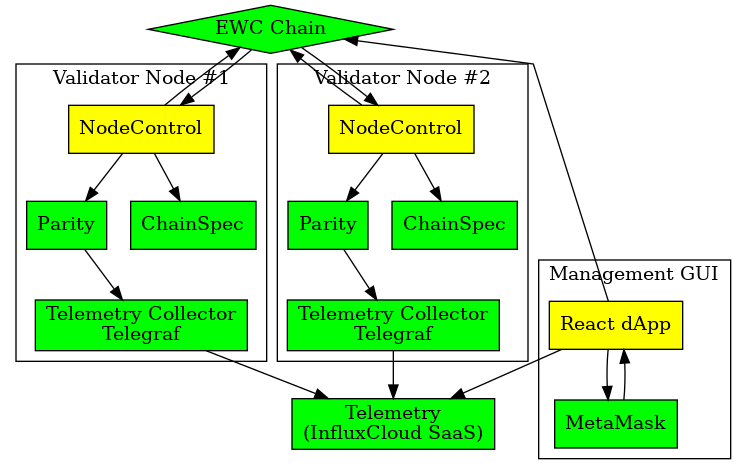
\includegraphics[width=0.85\textwidth,keepaspectratio]{./images/sys-diagram.png}
	\caption{Validator System Design}
	\label{fig:sysdesign}
\end{figure}

\subsection{System Components}
\label{components}

These system components are tailor made or where developed for the validator network.

\subsubsection{NodeControl}

A small deamon that will carry out updates on behalf of NetOps. See \ref{nodecontrol}.

\subsection{Other Components}

These components are standardize open-source components.

\subsubsection{Telemetry Collector}

The system uses Telegraf to collect the telemetry from on the nodes. This collected data is then send via the InfluxDB wire protocol to the also locally running telemetry signer.

\subsubsection{Telemetry SaaS Backend}

To gather and visualize the telemetry a SaaS provider is used.

\subsubsection{Blockchain Client}

The blockchain client is the main component of the system as it provides the connection to the blockchain and also carries out signing and validation duties. 
The probably used software will be Parity-Ethereum from Parity Tech running the AURA Proof-of-Authority engine.


\newpage
\section{NodeControl}
\label{nodecontrol}

NodeControl is a small management application that runs on each validator node. It is in charge of carrying out simple update tasks.
It will listen to the local blockchain client via the HTTP RPC interface. 
The ethereum address of the validator account is used as a node identifier. NodeControl will only act on events directly directed to its assigned address.
This allows granular deployment of updates. \\

The trigger process is shown in Fig. ~\ref{fig:nctrigger}.


\begin{figure}[ht]
	\centering
    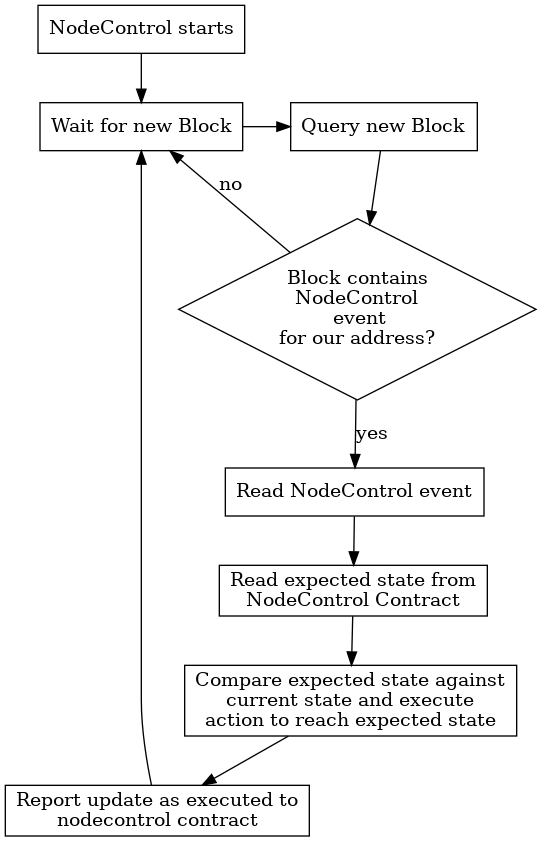
\includegraphics[height=0.65\textheight,keepaspectratio]{./images/nodecontrol.png}
	\caption{NodeControl Trigger Process}
	\label{fig:nctrigger}
\end{figure}

\newpage

\newpage
\section{Genesis Network}

The Genesis Network is a special set of validators and full nodes that will be used during launch. Hosts of the genesis network will be geographically distributed across different AWS regions. These regions will be linked via VPC peering, so traffic inside the genesis network is not public facing. \\

The genesis network will be run by the EnergyWeb Foundation.

\begin{figure}[ht]
	\centering
    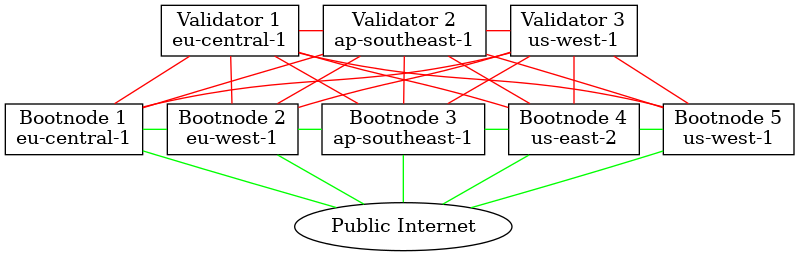
\includegraphics[width=0.85\textwidth,keepaspectratio]{./images/genesis-network.png}
	\caption{Genesis Network Layout}
	\label{fig:genesisnet}
\end{figure}

\subsection{Validators}

The genesis validators will be starting the chain and also their validator account addresses are hard coded as constructor arguments to the validator contract in the chain specification. The hosts running those validator nodes adhere to the same security standards as normal validators with the addition that they don't have any connection to the public internet blockchain wise. \\
The following outgoing traffic is permitted though an AWS NAT gateway:

\begin{itemize}
    \item DNS (53/UDP+TCP)
    \item HTTP (80/TCP) - mainly for sys updates
    \item HTTPS (443/TCP) - mainly for sending telemetry
\end{itemize}

Blockchain traffic is only allowed inside the AWS VPC to the Bootnodes. The validators will have a special configuration file for parity to facilitate that along with the following security group settings

\begin{itemize}
    \item Allow P2P traffic (30303/tcp+udp) inbound only from the bootnodes via RFC1918 inside the VPC
    \item Allow P2P traffic (30303/tcp+udp) outbound only to the bootnodes via RFC1918 inside the VPC
    \item Allow SSH traffic only inbound via a jump host inside the VPC over RFC1918
\end{itemize}

A preferred EC2 Instance type would be c5.xlarge. These nodes also don't have dedicated public IP's

\subsection{Bootnodes}

The genesis bootnodes are regular fullnodes (state pruned, no tracing, no fatdb, no warp).
They accept connections from the public internet and the validator VPC's on their blockchain P2P port.

Enode addresses of those bootnodes will be part of the general public chainspec.


\newpage
\section{Threat model}

This section describes potential attack vectors to the system and how they are either mitigated by the system design, automatic intervention or human intervention.

\subsection{Telemetry}

As telemetry needs to flow from the validators to a virtual single ingress point on the SaaS provider. It is not protected by decentralization.
This telemetry helps to detect abnormalities in the operation of the validators caused by either system malfunction or deliberate attacks.

\begin{description}
    \item[Sending tampered data] 
        If an attacker manages to disturb node operation, he might try to disguise this by sending normal looking telemetry to the telemetry ingress on behalf of the attacked node. NetOps would detect the faulty node with increased time delay as telemetry data would contradict actual node behavior. \\
        \textbf{Acknoledged:} The current SaaS system won't protect against this attack. 
    
    \item[Denial-of-Service against the telemetry ingress] 
        An attacker might try to bring down the telemetry ingress completely to "blind" the EWF NetOps team about the status of the validator network. \\
        \textbf{Acknoledged:} The SaaS provider should be able to handle an attack against his infrastructure. But this is not proofed.

    \item[Phishing for telemetry] 
        An attacker might try to receive telemetry from a node by re-routing telemetry traffic to an attacker system that mimics the ingress (DNS spoofing, MITM). The attacker can gain knowledge about for example the systems load patterns or how a system might respond to an attack. \\
        \textbf{Acknoledged:} The SaaS provider should be able to handle an attack against his infrastructure.
        
    \item[DNS-Spoof/MitM against GUI] 
        An attacker might manage to DNS Spoof/MitM the connection between the browser of a member from the NetOps team and the telemetry backend. This way the attacker could present a faked system state of the validator network to NetOps. \\
        \textbf{Acknoledged:} The SaaS provider is not able to provide signed data. Security relies on an untampered HTTPS connection.

    \item[Unauthorized access to telemetry data]
        Telemetry data should only be available to the EWF NetOps Team. An attacker might try to directly call the telemetry backend to receive the data. \\
        \textbf{Acknoledged:} The SaaS provider has to authenticate the users correctly.

\end{description}

\subsection{Node Control}

The Node control component is used to carry out updates to the validator nodes. These updates need to be legitimized by the EWF NetOps and GovOps teams.
The component has the potential to disable a node due to a faulty or malicious update .

\begin{description}
    \item[Send fake update event] 
        An attacker might try to fool the NodeControl into carrying out an update script that is not approved. \\
        \textbf{Prevention:} NodeControl will talk to its local blockchain client most of the time via IPC. 
        If it has to talk to outside nodes because the local client is down, it'll use incubed to verify responses.

    \item[Compromised Payload]
        An attacker might MitM traffic to any server NodeControl would download a payload from (mainly used for the chain spec file update process). \\
        \textbf{Containment:} Each update will have the SHA256 hash of its agreed payload on chain. The payload downloaded by NodeControl is verified against this hash. If the hashes don't match NodeControl will not carry out the command and report a faulty update to the NodeControl Contract.

\end{description}


\subsection{Other Attack Vectors}

This section consolidates attack vectors that are either not specific to a single component or targeted against miscellaneous components.

\begin{description}

    \item[Attack time servers] 
        The Aura PoA consensus algorithm highly depends on accurate system clocks. An attacker could try to manipulate the system clock by intercepting requests made by the operating system via NTP (Network Time Protocol). If the attacker shifts the system time by +block time or -block time the validator will start signing during the wrong slot. Other validators then won't accept that block because it is out-of-turn and vice-versa the manipulated node would mark all incoming blocks as invalid as from its point of view all other validators appear to be syncing out-of-turn. \\
        \textbf{Mitigation:} Some validator nodes should use high-precision hardware clocks such as GPS-based ones or DCF-77 clocks instead of NTP for their time source. This way not the whole network is affected. Normal operation could be restored by removing all non-precision-clock nodes from the network. This could mean reduced chain performance.

\end{description}


\newpage

\section{Validators run by Affiliates}

This section will go through the requirements needed to run a standard validator by an EWF affiliate.

\input{hardware.tex}
\subsection{Supported Operating Systems}

The following Linux-based Operating Systems are supported for running a authority node: 

\begin{itemize}
    \item Ubuntu Server 18.04 LTS
    \item Debian 9.8
    \item CentOS 7
\end{itemize}

Affiliates can apply for a certain operating system, but in order to keep a heterogeneous infrastructure EWF NetOps can instruct the Affiliate to use a specific operating system from the above list. 
The operating system must be installed according to the settings described in this document to qualify the host for becoming part of the authority network.


\subsection{Security Requirements}

Running an authority nodes requires raised awareness of host and node security as authorities are a main attack surface to disturb operation of the block chain.
The following security rules apply:

\begin{itemize}
    \item No services are permitted to run on the same host that are not part of the authority node package
    \item All incoming connections on all ports except SSH (22/tcp) and the P2P (30303/tcp+udp) port have to be firewalled on the host with DROP rules. To guarantee proper network etiquette, incoming ICMP has to be accepted.
    \item SSH access is only allowed for non-root users
    \item SSH access is only allowed through RSA keys
    \item Parity RPC endpoints (HTTP, WebSocket) have to be disabled for external use (only docker stack internal)
    \item System updates have to applied regularly and in a timely manner
    \item Regular run of rootkit detectors
\end{itemize}

Most of these rules will be provided in the following set up guides.
\input{connectivity.tex}
\input{aws-security.tex}

%\newpage
%\input{ssh.tex}
\newpage

\subsection{Setup Procedure}

To setup a new authority node read this whole document and then use this procedure to carry out the set up. The full process is shown in Figure ~\ref{fig:onboardflow}

\begin{enumerate}
    \item Choose hosting provider (on-premise or qualified cloud provider) and favored operating system
    \item Consult with EWF NetOps on location and operating system
    \item EWF NetOps will provide the location and OS to use, along with the official installation script for the chosen operating system
    \item Install operating system according to this document
    \item Deploy blockchain node using the script given by NetOps 
    \item Contact EWF NetOps to confirm installation and incoming telemetry
    \item Send the validator account information to the EWF Governance team
\end{enumerate}





\newpage
\input{os-install.tex}
\newpage
\section{Telemetry}

Authority nodes have to send automatic telemetry data to NetOps. This helps detecting attacks or other network disturbances early.
The following telemetry is collected and send to the telemetry SaaS provider:

\begin{itemize}
    \item CPU usage
    \item Memory usage
    \item Disk usage
    \item Number of connected blockchain peers
    \item Current block information (hash, number of tx, blocktime)
    \item Network throughput
    \item Network error rate
    \item Service status for SSH, Docker and the Parity container
    \item Statisatics per docker container
\end{itemize}



\end{document}
